\section{Estensione del Modello}
In questa sezione verrano descritte le modifiche e le aggiunte effettuate al modello base,
% TODO: riscrivere
ma prima verrano evidenziate le limitazioni e le mancanze del modello anche rispetto allo stato dell'arte.

Molte assunzioni sono poco realistiche come la velocità costante dei pedoni, tutte le strade a senso unico e l'assenza di interazioni nelle
intersezioni.
%
Inoltre viene assunto che tutti gli agenti conoscano il percorso più breve per il rifugio.
%
Un'altra limitazione riguarda le interazioni tra i vari tipi di agenti.
Questo modello considera esclusivamente le interazioni auto-auto
tramite il modello General Motors, ma non prevede nessuna interazione pedone-pedone o pedone-auto.

% TODO: riscrivere
Come è stato appena descritto le interazioni tra gli agenti
hanno un ampio margine per essere ?rappresentate?, in particolare ci si concentrerà sulle interazioni nelle intersezioni
introducendo meccanismi di coordinazione tra i vari tipi di agente. Inoltre la velocità dei pedoni verrà modificata in base alla congestione
in modo da poter rappresentare uno scenario più realistico.

\subsection{Rete Stradale}
Prima di descrivere le varie aggiunte in questa sezione verrannò elencate le varie modifiche che sono state effettuate alla rete stradale.

Tutte le strade della rete sono state considerate come strade locali secondo il \textcite{seaside2010tsp},
ovvero strade a doppio senso e a una corsia con una larghezza variabile da 7.3 m a 9 m e opzionalmente
un marciapiedie per ogni lato della strada con una larghezza fissa di 1.5 m.
%
È stato assunto che tutte le strade abbiano marciapiedi su entrambi i lati e che la larghezza sia fissata al valore minimo.

% TODO: espandere
Sono stati associati gli stop alle strade collegate ad un intersezioni.

\subsection{Speed Variability dei Pedoni}
Riassunto stato dell'arte per la speed variability e survey di modelli macroscopici sui diagrammi fondamentali.

È stata introdotta una variabilità nella velocità di camminata per i pedoni utilizzando il modello di Weiddman con una \textit{free flow speed} di 1.34 m/s
e una \textit{jam density} di 5.4 p/m².
Il calcolo della densità è stato effettuato considerando un'area di ricerca di 4 m x 1.5 m di fronte al pedone,
come in \textcite{goto2012tsunami, wang2021novel}.

I pedoni nel caso in cui sono presenti anche auto, procedono esclusivamente sui marciapiedi, altrimenti occupano tutta la strada.

Spiegare modello di weidmann.

\newpage

\subsection{Gestione degli Intersezioni}
Per la gestione delle intersezioni sono stati considerati esclusivamente gli incroci a 4 strade e trattati come intersezioni di tipo AWSC (All Way Stop Controlled) o TWSC (Two Way Stop controlled).

% TODO: riscrivere, un po' confuso
Tramite l'utilizzo di OpenStreetMap e GoogleMaps, sono state estratte manualmente le informazioni circa la posizione e nel case dei TWSC la direzione
di precedenza di tali tipi di incroci per la citta di Seaside, ottenendo la seguente (Fig. \ref{fig:intersections}).

\begin{figure}
    \centering
    \begin{subfigure}{0.475\textwidth}
        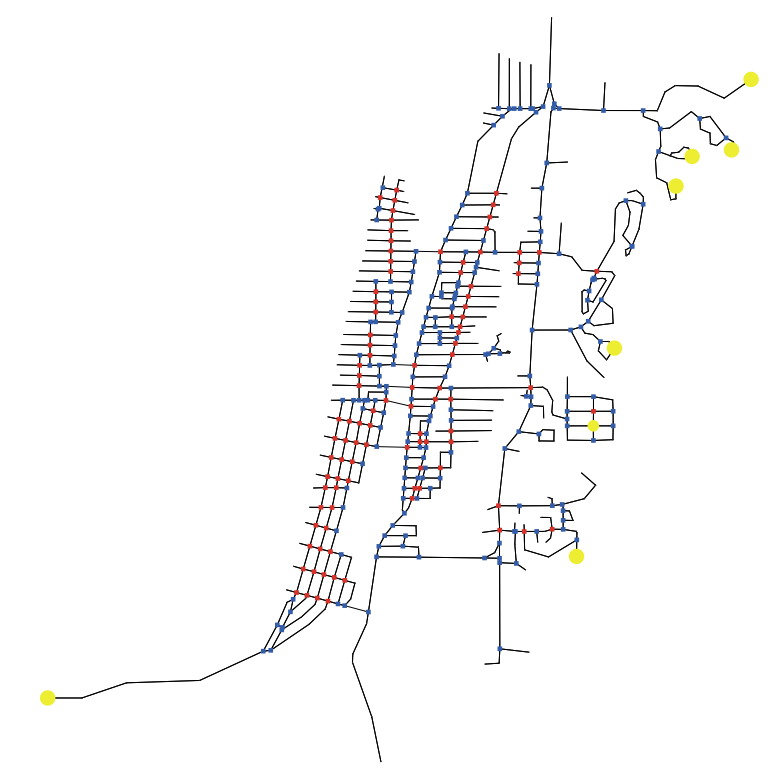
\includegraphics[width=\textwidth]{images/intersections}
        \caption{intersezioni classificate per numero di strade: verde a 4 strade (98 nodi) e grigio a 3 strade (206 nodi).}
        \label{fig:intersections}
    \end{subfigure}
    \hfill
    \begin{subfigure}{0.475\textwidth}
        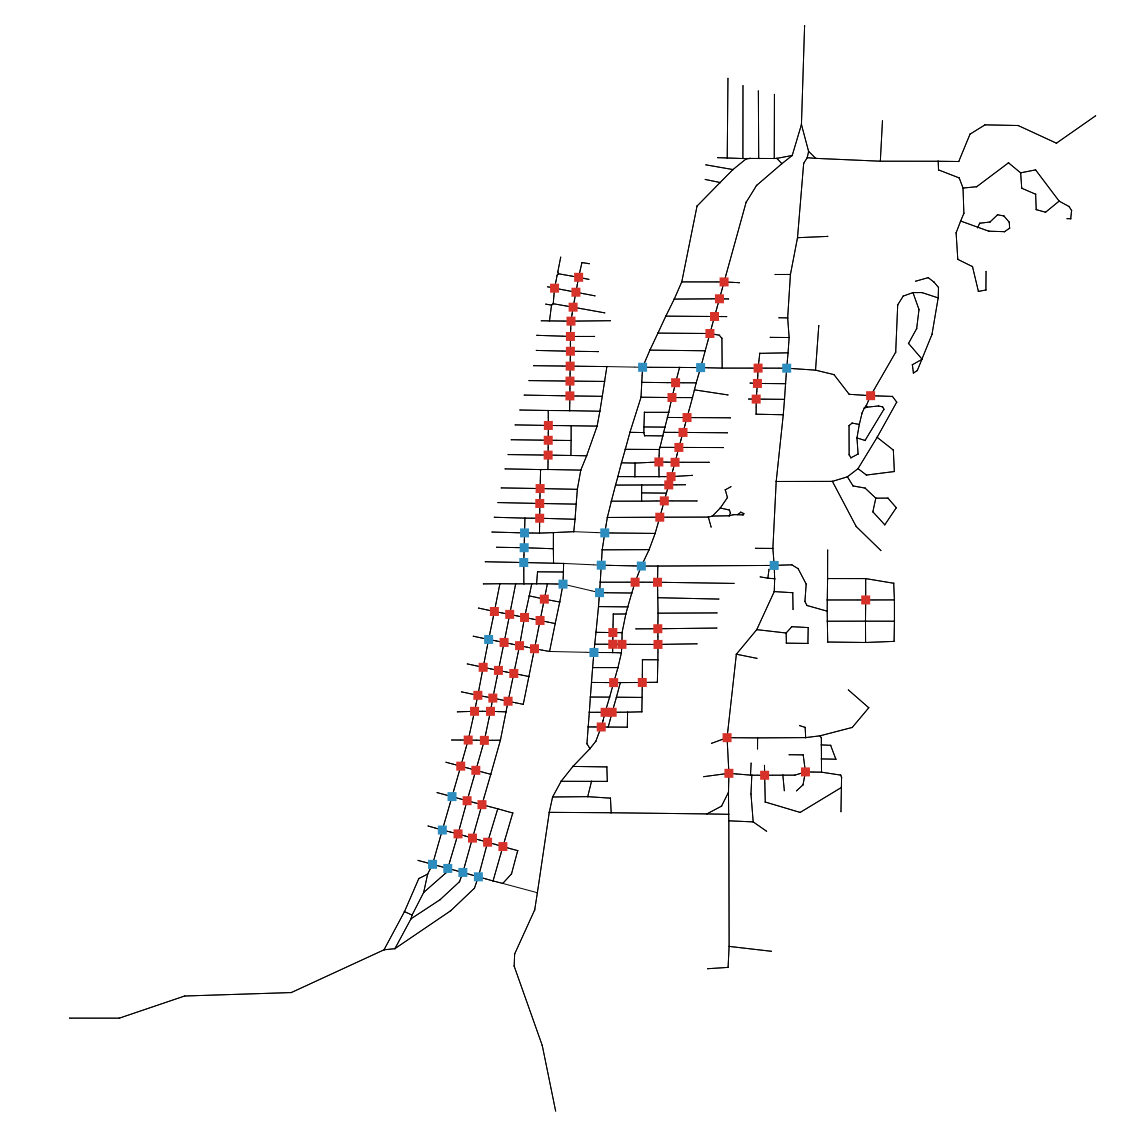
\includegraphics[width=\textwidth]{images/int_type}
        \caption{intersezioni a 4 strade classificate in base al tipo: AWSC in blu (20 nodi) e TWSC in rosso (78 nodi).}
        \label{fig:intersections_types}
    \end{subfigure}
    \caption{Tipi di intersezioni.}
\end{figure}

Inoltre nelle intersezioni è stata introdotta una zona di attraversamento per la gestione delle interazioni tra auto e pedoni.
È stato assunto che gli incroci abbiano lunghezza e larghezza pari alla larghezza della strada (10.3 m).
Dal momento che la rappresentazione della strada è network-based è stato deciso che
la zona iniza prima dell'incrocio e finisce dopo dell'incrocio a una distanza pari alla metà della larghezza (5.15 m) (Fig. \ref{fig:crossing-area}).

\begin{figure}[ht]
    \centering
    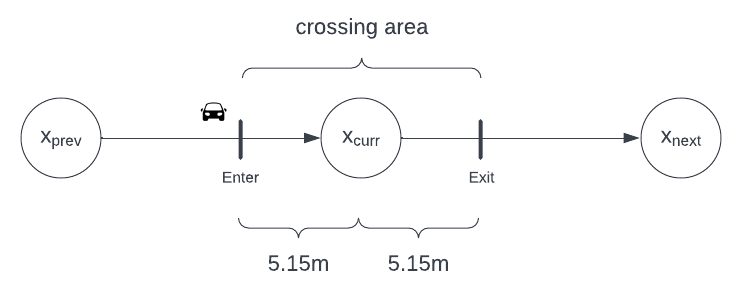
\includegraphics[width=0.5\textwidth]{images/crossing_area}
    \caption{Zona di attraversamento di un'intersezione.}
    \label{fig:crossing-area}
\end{figure}

\newpage
Per rappresentare l'attraversamento dei pedoni e delle auto sono state aggiunte le seguenti informazioni ad ogni intersezione $i$ a 4 strade:
\begin{itemize}
    \item $C_{i, j}$ = numero di pedoni che stanno usando l'attraversamento pedonale che si trova sulla strada che va dall'incrocio $i$ all'incrocio $j$.
    \item $\textit{Arrival}_i$ = coda delle auto nella zona di attraversamento ordinate per tempo di arrivo.
    \item $\textit{Crossing}_i$ = insieme delle auto che possono passare contemporaneamente.
    \item $\textit{Stops}_i$ = insieme delle intersezioni $j$ collegate a $i$ in cui è presente uno stop nella strada $(i, j)$.
\end{itemize}

% Inoltre per i TWSC nelle intersezioni la presenza degli stop viene segnata, mediante una lista con il numero dell'intersezioni interessate.

Per stabilire la posizione all'interno della rete stradale, le precedenze e la direzione della prossima intersezione per ogni agente $x$
vengono definite:
\begin{itemize}
    \item $x_{prev}$ l'intersezione precendente
    \item $x_{curr}$ l'intersezione corrente
    \item $x_{next}$ la prossima intersezione
    \item $x_{side} \in \{ \textit{left}, \textit{right} \}$  il lato di marciapiede (solo pedoni)
    \item $x_{xdir} \in \{\textit{left}, \textit{straight}, \textit{right}\}$ la direzione verso $x_{next}$
\end{itemize}

\newpage
\subsubsection{Pedoni}
% Dato un pedone $x$ si definiscono $x_{prev}$ l'intersezione precendente, $x_{curr}$ l'intersezione corrente e $x_{next}$ la prossima intersezione.

Data la tripla ($x_{prev}$, $x_{curr}$, $x_{next}$) viene associata ad ogni intersezione collegata a $x_{curr}$ la direzione per raggiungerla seguendo il senso orario a partire da $x_{prev}$,
per cui $I_d$ indica l'intersezione nella direzione $d \in \{\textit{origin}, \textit{left}, \textit{straight}, \textit{right}\}$.
%
La direzione associata all'intersezione $x_{next}$ è quella dove è diretto il pedone e viene identificata da $x_{dir}$.

Quando un pedone $x$ entra nella zona di attraversamento di $x_{curr}$ dall'intersezione $x_{prev}$ e si trova sul marciapiede $x_{side}$
ha tre direzioni in cui poter andare: \textit{left}, \textit{straight}, \textit{right} (Fig. \ref{fig:pedestria-crossing}):
\begin{itemize}
    \item Se $x_{dir} = \textit{straight}$ e $x_{side} = \textit{side}$ viene incrementato $C_{x_{curr}, I_{\textit{side}}}$ di 1.
    \item Se $x_{dir} = \textit{side}$ e $x_{side} \neq \textit{side}$ viene incrementato $C_{x_{curr}, I_{\textit{origin}}}$ di 1.
    \item Se  $x_{dir} = \textit{side}$ e $x_{side} = \textit{side}$ non viene alterato nessun contatore.
\end{itemize}

Quando il pedone finisce di attraversare il contatore corrispondente viene decrementato di 1.


\begin{figure}[ht]
    \centering
    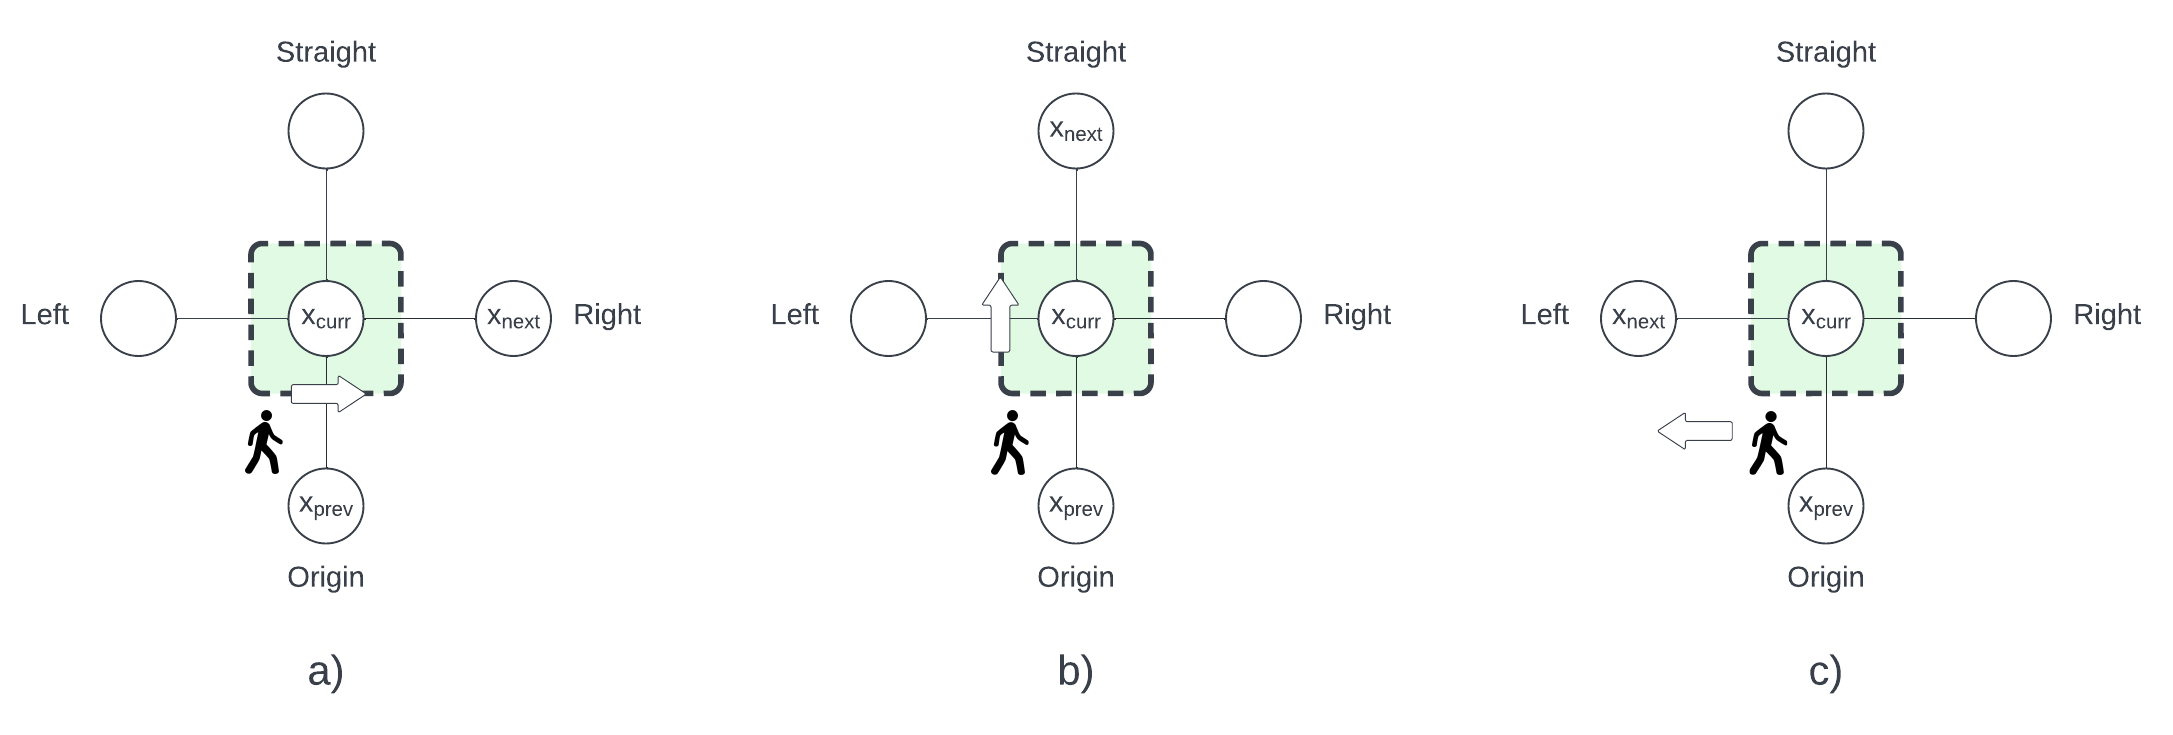
\includegraphics[width=\textwidth]{images/pedestrian_crossing}
    \caption{
        Esempio dei tre casi di attraversamento dal punto di vista del pedone che si trova sul marciapiede sinistro.
        a) il pedone si trova sul lato sinistro e attraversa sul link collegato a origin.
        b) il pedone attraverso sul lato sinistro dell'incrocio, quindi sul link collegato a left.
        c) il pedone segue il marciapiede sulla sinistra senza attraversare.
    }
    \label{fig:pedestria-crossing}
\end{figure}


\subsubsection{Auto}
Quando un auto $x$ raggiunge la zona di attraversamento dell'intersezione $i$ viene aggiunta alla coda $\textit{Arrival}_i$ che
determina l'ordine di arrivo delle auto. In base al tipo di intersezione viene schedulata e una volta avuto il via libera
viene aggiunta a $\textit{Crossing}_i$ e rimossa una volta lasciato l'incrocio.

Le auto quando raggiungono la zona di attraversamento vengono aggiunte alla coda $\textit{Arrival}_i$ e schedulate
in base al tipo d'intersezione (Sec. \ref{subsubsec:precedenze}), una volta avuto il via libera le auto sono aggiunte a $\textit{Crossing}_i$
e rimosse una volta lasciato l'incrocio.
%
Se ci sono pedoni che stanno attraversando le strade $(x_{curr}, x_{next})$ e $(x_{prev}, x_{curr})$ l'auto dovrà attendere,
quindi potrà passare se e solo se $C_{x_{curr},x_{prev}}$ = 0 e $C_{x_{curr},x_{next}}$ = 0 (Fig. \ref{fig:auto-ped-crossing}).

\begin{figure}[ht]
    \centering
    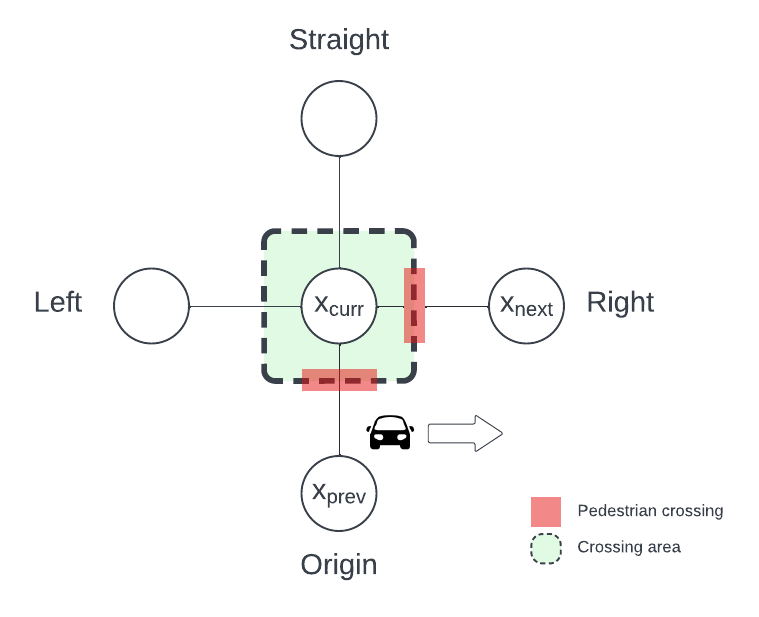
\includegraphics[width=0.45\textwidth]{images/crossing_auto_ped_crossing}
    \caption{Esempio degli attraversamenti pedonali (in rosso) che vanno controllati
        per poter passare data la tripla ($x_{prev}$, $x_{curr}$, $x_{next}$) di un auto $x$.}
    \label{fig:auto-ped-crossing}
\end{figure}

\subsubsection{AWSC}
\label{subsubsec:precedenze}
Nelle intersezioni di tipo AWSC la prima auto che arriva ha la precedenza sulle altre auto e deve aspettare eventuali pedoni come spiegato in precedenza.
Inoltre lo scenario in cui 4 auto arrivano contemporaneamente non è stato considerato poiché poco probabile.

La risoluzione delle precedenze avviene tra le auto che arrivano a un'intersezione allo stesso tempo.
L'auto che ha la destra libera viene considerata provenire da \textit{origin} e dal suo punto di riferimento
vengono identificate le direzioni di provenienza delle altre auto.

Basandosi sulle direzioni di provenienza delle auto e sulle rispettive destinazioni viene verificato
in senso orario (\textit{origin} $\rightarrow$ \textit{left} $\rightarrow$ \textit{straight})
quali auto possono passare contemporaneamente o meno (Tab. \ref{tab:origin-left}, Tab. \ref{tab:origin-straight}, Tab. \ref{tab:origin-left-straight}).


\begin{table}[ht]
    \centering
    \begin{tabular}{|c|c|c|}
        \hline
        \textbf{Car1: Origin} & \textbf{Car2: Left} \\ \hline
        Left                  & Left                \\ \hline
        Right                 & Right               \\ \hline
        Right                 & Straight            \\ \hline
        Straight              & Right               \\ \hline
    \end{tabular}
    \caption{Tutte le possibili combinazioni di destinazione delle due auto che permettono
        di passare contemporaneamente nel caso in cui arrivano rispettivamente da \textit{origin} e \textit{left}.}
    \label{tab:origin-left}
\end{table}

\begin{table}[ht]
    \centering
    \begin{tabular}{|c|c|c|}
        \hline
        \textbf{Car1: Origin} & \textbf{Car2: Straight} \\ \hline
        Left                  & Right                   \\ \hline
        Right                 & Left                    \\ \hline
        Right                 & Right                   \\ \hline
        Straight              & Right                   \\ \hline
    \end{tabular}
    \caption{Tutte le possibili combinazioni di destinazione delle due auto che permettono
        di passare contemporaneamente nel caso in cui arrivano rispettivamente da \textit{origin} e \textit{straight}.}
    \label{tab:origin-straight}
\end{table}

\begin{table}[ht]
    \centering
    \begin{tabular}{|c|c|c|}
        \hline
        \textbf{Car1: Origin} & \textbf{Car2: Left} & \textbf{Car3: Straight} \\ \hline
        Right                 & Left                & Right                   \\ \hline
        Left                  & Right               & Left                    \\ \hline
        Right                 & Right               & Right                   \\ \hline
        Straight              & Right               & Right                   \\ \hline
    \end{tabular}
    \caption{Tutte le possibili combinazioni di destinazione delle tre auto che permettono
        di passare contemporaneamente nel caso in cui arrivano rispettivamente da \textit{origin}, \textit{left} e \textit{straight}.}
    \label{tab:origin-left-straight}
\end{table}

\subsubsection{TWSC}
Nel caso in cui l'intersezione è di tipo TWSC vengono identificate due vie: quella principale che ha la precedenza e quella
secondaria in cui sono presenti gli stop.

A differenza dell'intersezioni AWSC, l'ordine di precedenza non importa poiché possono passare al più due auto alla volta
che si trovano l'una di fronte all'altra.
Quindi viene scelta casualmente come riferimento una delle due auto che viene considerata provenire da \textit{origin}, mentre
l'altra da \textit{straight}.
%
Una volta che la via principale è libera viene gestita nello stesso modo quella secondaria.

Per verificare se le due auto possono passare contemporaneamente si procede come già visto per il caso origin-straight (Tab. \ref{tab:origin-left-straight}).
